\documentclass[10pt]{beamer}

\usetheme{Madrid}
\usecolortheme{default}

% Base packages
%\usepackage{helvet}
\usepackage{amsmath,amssymb,mathtools,subcaption}
\usepackage{tikz,pgfplots,tabularx,booktabs}
\usepackage{listings}
\usepackage{xcolor}

% Font settings
\renewcommand{\familydefault}{\sfdefault}

% TikZ libraries
\usetikzlibrary{calc,positioning,backgrounds,decorations.pathreplacing}
\pgfplotsset{compat=1.14}

% Colors
\definecolor{deepblue}{RGB}{42,39,155}
\definecolor{lightpink}{RGB}{255,240,240}
\definecolor{lightgreen}{RGB}{240,255,240}
\definecolor{lightyellow}{RGB}{255,255,240}
\definecolor{codegray}{RGB}{245,245,245}
\definecolor{codegreen}{rgb}{0,0.6,0}
\definecolor{codepurple}{rgb}{0.58,0,0.82}

% Beamer settings
\setbeamercolor{title}{fg=white,bg=deepblue}
\setbeamercolor{frametitle}{fg=white,bg=deepblue}
\setbeamercolor{section in head/foot}{fg=white,bg=deepblue}

% Code listing settings
\lstdefinelanguage{iPython}{
  language=Python,
  morekeywords={as,assert,async,await,break,class,continue,def,del,elif,else,
    except,finally,for,from,global,if,import,in,is,lambda,nonlocal,not,or,
    pass,raise,return,try,while,with,yield,True,False,None},
  sensitive=true,
  morecomment=[l]{\#},
  morestring=[b]',
  morestring=[b]"
}

\lstset{
    language=iPython,
    basicstyle=\ttfamily\small,
    backgroundcolor=\color{codegray},
    breaklines=true,
    showstringspaces=false,
    commentstyle=\color{codegreen},
    keywordstyle=\color{blue},
    stringstyle=\color{codepurple},
    numbers=none,
    frame=none
}

\setbeamertemplate{footline}[text line]{%
  \parbox{\linewidth}{\vspace*{-8pt}
  %\hfill\href{https://github.com/chang-ye-tu/fin}{https://github.com/chang-ye-tu/fin}
    \hfill
   ~~ \insertframenumber / \inserttotalframenumber~~~~~~~~~}}
\setbeamertemplate{navigation symbols}{}%[only frame symbol]

\definecolor{foo}{rgb}{.2,.2,.7}
\AtBeginSection[]{
  \begin{frame}
  \vfill
  \centering
  \begin{beamercolorbox}[sep=8pt,center,shadow=true,rounded=true]{section page}
    \usebeamerfont{title}%
    {\color{foo} \insertsectionhead}\par%
  \end{beamercolorbox}
  \vfill
  \end{frame}
}

\title{Introduction to Financial Models \\ Lecture 02: Surprises \& Paradoxes II}
\author{}
\date{}

\begin{document}

\begin{frame}
\titlepage
\end{frame}

\subsection*{Outline}
\begin{frame}
  \tableofcontents
\end{frame}

\section{Coin Rotation Paradox}

\begin{frame}
\begin{center}
  \href{https://www.youtube.com/watch?v=FUHkTs-Ipfg}{\textbf{The 1982 SAT Question Everyone Got Wrong}}
  \vspace{1cm}

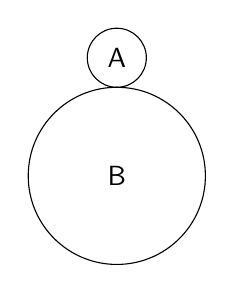
\begin{tikzpicture}[scale=.5]
    % Draw circle B (larger circle)
  \draw (0,0) circle (2.25cm);
    \node at (0,0) {B};
    
    % Draw circle A (smaller circle)
    \draw (0,3) circle (0.75cm);
    \node at (0,3) {A};
\end{tikzpicture}

\vspace{.5cm}

The radius of circle A is $\frac{1}{3}$ of the radius of circle B. Circle A rolls\\
around circle B one trip back to its starting point. How\\
many times will circle A revolve in total?

\vspace{.5cm}

\begin{tabular}{l@{\hspace{2em}}l@{\hspace{2em}}l@{\hspace{2em}}l@{\hspace{2em}}l}
  (a) $\frac{3}{2}$ & (b) 3 & (c) 6 & (d) $\frac{9}{2}$ & (e) 9
\end{tabular}
\end{center}

\vspace{.5cm}

\end{frame}

\section{Braess Paradox}

\begin{frame}

\end{frame}

\end{document}
